% Copyright 2005-2016 Airbus-EDF-IMACS-Phimeca
% Permission is granted to copy, distribute and/or modify this document
% under the terms of the GNU Free Documentation License, Version 1.2
% or any later version published by the Free Software Foundation;
% with no Invariant Sections, no Front-Cover Texts, and no Back-Cover
% Texts.  A copy of the license is included in the section entitled "GNU
% Free Documentation License".
\renewcommand{\filename}{docUC_StocProc_NonStationaryCovarianceFunction_Estimation.tex}
\renewcommand{\filetitle}{UC : Estimation of a non stationary covariance function}

% \HeaderNNIILevel
% \HeaderIILevel
\HeaderIIILevel

\index{Stochastic Process!Covariance Model}

Let $X: \Omega \times \cD \rightarrow \Rset^d$  be a multivariate  normal process of dimension $d$ where $\cD \in \Rset^n$. $X$ is supposed to be a second order process and we note  $C : \cD \times  \cD \rightarrow  \mathcal{M}_{d \times d}(\mathbb{R})$ its covariance function.\\

The objective of this use case is to estimate $C$ from several fields generated by the process $X$. We suppose that the process is not stationary. \\

We denote $(\vect{t}_0, \dots, \vect{t}_{N-1})$ the vertices of the common mesh $\cM$ and $(\vect{x}_0^k, \dots, \vect{x}_{N-1}^k)$ the associated values of the field $k$. We suppose that we have $K$ fields.\\

We recall that the covariance function $C$ writes:
\begin{equation}\label{covFunc}
  \forall (\vect{s}, \vect{t}) \in \cD \times \cD, \quad C(\vect{s}, \vect{t}) = \Expect{\left(X_{\vect{s}}-m(\vect{s})\right)\left(X_{\vect{t}}-m(\vect{t})\right)^t}
\end{equation}
where the mean function $m: \cD \rightarrow \Rset^d$ is defined by :
\begin{equation}\label{meanFunc}
  \forall  \vect{t}\in \cD , \quad m(\vect{t}) = \Expect{X_{\vect{t}}}
\end{equation}

First, OpenTURNS estimate the covariance function $C$ on the vertices of the mesh $\cM$. At each vertex $\vect{t}_i \in \cM$, we use the empirical mean estimator applied to the $K$ fields  to estimate :
\begin{enumerate}
\item  $m(\vect{t}_i)$ at the vertex $\vect{t}_i$:
  \begin{equation}\label{meanestim}
    \displaystyle  \forall \vect{t}_i \in \cM, \quad m(\vect{t}_i) \simeq \frac{1}{K} \sum_{k=1}^{K} \vect{x}_i^k
  \end{equation}

\item $C(\vect{t}_i, \vect{t}_j)$ at the vertices $(\vect{t}_i, \vect{t}_j)$:
  \begin{equation}\label{covEstm}
    \displaystyle \forall (\vect{t}_i, \vect{t}_j) \in \cD \times \cD, \quad C(\vect{t}_i, \vect{t}_j) \simeq \frac{1}{K} \sum_{k=1}^{K} \left( \vect{x}_i^k -  m(\vect{t}_i) \right) \left( \vect{x}_j^k -  m(\vect{t}_j) \right)^t
  \end{equation}
\end{enumerate}
Then,  OpenTURNS builds a covariance function defined on $\cD \times \cD$  which is a  piecewise constant function defined on $\cD \times \cD$ by:
\begin{align*}
  \forall (\vect{s}, \vect{t}) \in \cD \times \cD, \, C^{stat}(\vect{s}, \vect{t}) =  C(\vect{t}_k, \vect{t}_l)
\end{align*}
where $k$ is such that $\vect{t}_k$ is the  vertex of $\cM$ the nearest to $\vect{s}$ and $\vect{t}_l$ the nearest to $\vect{t}$.\\


OpenTURNS uses the object \textit{NonStationaryCovarianceModelFactory} wich creates a \newline \textit{UserDefinedCovarianceModel}.\\


\requirements{


  \begin{description}
  \item[$\bullet$] a set of fields {\itshape myFieldSample}
  \item[type:]  ProcessSample
  \end{description}

}
{
  \begin{description}
  \item[$\bullet$] a factory {\itshape myFactory}
  \item[type:]  NonStationaryCovarianceModelFactory
  \end{description}

  \begin{description}
  \item[$\bullet$] a covariance model: {\itshape  myEstimatedModel}
  \item[type:]  UserDefinedCovarianceModel
  \end{description}
}

\textspace\\
Python script for this Use Case:

\inputscript{script_docUC_StocProc_NonStationaryCovarianceFunction_Estimation}

In the following example, we illustrate the estimation of the non stationary covariance model $C : \cD \times [-4, 4] \rightarrow  \Rset $ defined by:
\begin{align}
  \displaystyle C(s,t) = \exp\left(-\dfrac{4|s-t|}{1+s^2+t^2}\right)
\end{align}
The domaine $\cD$ is  discretized on a mesh $\cM$ which is a time grid with 64 points.\\
We build a normal process $X: \Omega \times [-4, 4]  \rightarrow \Rset$ with zero mean and $C$ as covariance function. OpenTURNS discretizes the covariance model $C$ using $C(t_k, t_\ell)$ for each $(t_k, t_\ell)\in \cM \times \cM$.\\
We get a $N=10^3$ fields from the process $X$ from wich we estimate the covariance model $C$. The Figure \ref{NonStatCovEstim} draws the iso contours of the estimated model compared to the theoretical one.


\begin{figure}[H]
  \begin{center}
    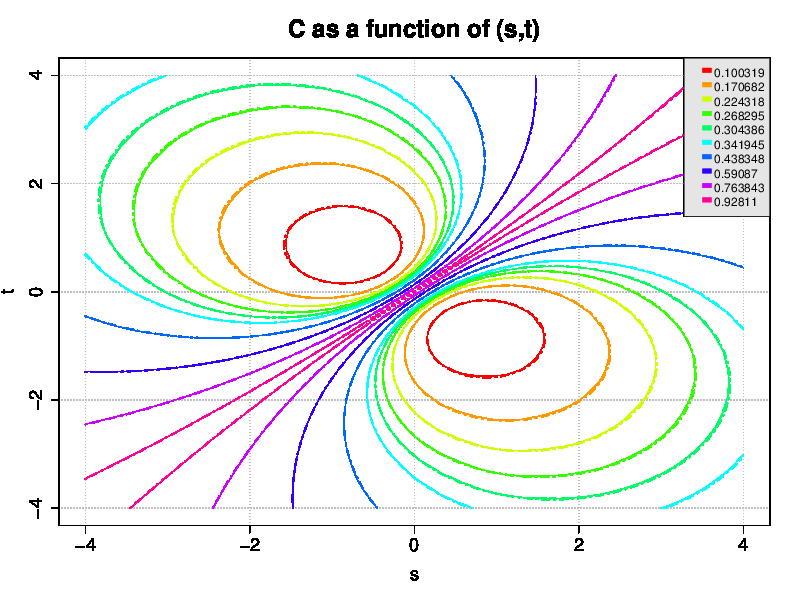
\includegraphics[width=7cm]{Figures/NonStatCovFuncEstim.png}
    \caption{Estimation of a non stationary covariance model of a scalar process on $[-4, 4]$.}
    \label{NonStatCovEstim}
  \end{center}
\end{figure}
